% Draft evaluation subsections for the SCALE paper. Generated by analysis/latex_export.py;
% edit freely after copying into the paper. Requires: % Generated by analysis/latex_export.py -- do not edit by hand.
% % Generated by analysis/latex_export.py -- do not edit by hand.
% % Generated by analysis/latex_export.py -- do not edit by hand.
% \input{macros} in the preamble; every macro is prefixed with \scale.
% Each line ends with a comment saying what the value means, measures or represents
% (descriptions live in analysis/macro_docs.py). Percentages are relative differences
% unless stated; 'design level' means one value per mix design, repeats averaged.
\providecommand{\xspace}{}
\newcommand{\scaleNEvaluations}{7{,}944\xspace}                          % number of MoST pass/fail SLA evaluations analysed (all runs, after removing exact copies)
\newcommand{\scaleNMixRuns}{301\xspace}                                  % number of mix runs (MoST searches on request mixes)
\newcommand{\scaleNDesigns}{114\xspace}                                  % number of distinct mix designs (model x test x composition); unit of the frequentist tests
\newcommand{\scaleNRepeatRuns}{270\xspace}                               % number of mix runs that belong to designs measured more than once
\newcommand{\scaleNRepeatDesigns}{83\xspace}                             % number of mix designs measured more than once (stability check)
\newcommand{\scaleNDuplicates}{114\xspace}                               % number of byte-identical copies of a run found in the archive and counted once
\newcommand{\scaleNPureRuns}{360\xspace}                                 % number of pure-class runs (one request class per MoST search)
\newcommand{\scaleQHatFreq}{\ensuremath{-}0.91\xspace}                   % power-mean exponent q of the combination law, profile-likelihood estimate (q=-1 harmonic, 0 geometric, +1 arithmetic)
\newcommand{\scaleQFreqLo}{\ensuremath{-}0.98\xspace}                    % lower bound of the 95 % profile-likelihood confidence interval of q
\newcommand{\scaleQFreqHi}{\ensuremath{-}0.84\xspace}                    % upper bound of the 95 % profile-likelihood confidence interval of q
\newcommand{\scaleHarmonicWinShare}{97\,\%\xspace}                       % share of mix runs for which the harmonic prediction is closer to the measurement than the arithmetic one
\newcommand{\scaleCalibSlope}{0.96\xspace}                               % slope of the regression log(measured mix capacity) ~ log(harmonic prediction); 1 = correct scaling
\newcommand{\scaleCalibSlopeLo}{0.90\xspace}                             % lower bound of the 95 % confidence interval of the calibration slope (cluster-robust by model)
\newcommand{\scaleCalibSlopeHi}{1.02\xspace}                             % upper bound of the 95 % confidence interval of the calibration slope
\newcommand{\scaleCalibRsq}{0.97\xspace}                                 % R^2 of the calibration regression on the log scale
\newcommand{\scaleBiasFreq}{\ensuremath{-}3.0\,\%\xspace}                % mean departure of measured mix capacity from the harmonic prediction, frequentist, designs as units
\newcommand{\scaleBiasFreqLo}{\ensuremath{-}6.9\,\%\xspace}              % lower bound of the 95 % confidence interval of BiasFreq
\newcommand{\scaleBiasFreqHi}{+1.0\,\%\xspace}                           % upper bound of the 95 % confidence interval of BiasFreq
\newcommand{\scaleBiasTostP}{0.001\xspace}                               % p-value of the TOST equivalence test of the bias against +-10 % (small = practically zero)
\newcommand{\scaleArithMeanErr}{\ensuremath{-}53\,\%\xspace}             % mean error of the arithmetic-mean law (measured vs predicted mix capacity, design level); negative = overestimates
\newcommand{\scaleGeomMeanErr}{\ensuremath{-}39\,\%\xspace}              % mean error of the geometric-mean law (design level); negative = overestimates
\newcommand{\scaleBoundsIn}{294\xspace}                                  % number of mix runs whose capacity lies between their slowest and fastest class
\newcommand{\scaleBoundsN}{301\xspace}                                   % number of mix runs checked for boundedness
\newcommand{\scaleBoundsShare}{97.7\,\%\xspace}                          % share of mix runs within the capacity range of their classes
\newcommand{\scaleAboveArith}{0\xspace}                                  % number of mix runs whose capacity exceeds the arithmetic mean of their classes
\newcommand{\scaleQHatBayes}{\ensuremath{-}0.96\xspace}                  % power-mean exponent q, Bayesian posterior median (free-q model)
\newcommand{\scaleQBayesLo}{\ensuremath{-}1.02\xspace}                   % lower bound of the 95 % credible interval of q
\newcommand{\scaleQBayesHi}{\ensuremath{-}0.88\xspace}                   % upper bound of the 95 % credible interval of q
\newcommand{\scaleBiasBayes}{\ensuremath{-}5.5\,\%\xspace}               % pooled bias delta_0 of mixes w.r.t. the harmonic law, Bayesian posterior median
\newcommand{\scaleBiasBayesLo}{\ensuremath{-}9.9\,\%\xspace}             % lower bound of the 90 % credible interval of delta_0
\newcommand{\scaleBiasBayesHi}{\ensuremath{-}1.0\,\%\xspace}             % upper bound of the 90 % credible interval of delta_0
\newcommand{\scaleBiasBayesPRope}{92\,\%\xspace}                         % posterior probability that |delta_0| < 10 % (region of practical equivalence)
\newcommand{\scalePredFree}{+1.7\xspace}                                 % out-of-sample log predictive density of the free-q law minus that of the harmonic law (higher = better)
\newcommand{\scalePredFreeSE}{3.3\xspace}                                % standard error of PredFree
\newcommand{\scalePredGeom}{\ensuremath{-}264.5\xspace}                  % out-of-sample log predictive density of the geometric law minus that of the harmonic law
\newcommand{\scalePredGeomSE}{24.8\xspace}                               % standard error of PredGeom
\newcommand{\scalePredArith}{\ensuremath{-}441.4\xspace}                 % out-of-sample log predictive density of the arithmetic law minus that of the harmonic law
\newcommand{\scalePredArithSE}{38.1\xspace}                              % standard error of PredArith
\newcommand{\scaleSdMixMIT}{6\,\%\xspace}                                % posterior SD of the design effect (departure of a mix design from the harmonic law), MIT (2-minute instantaneous test), as %
\newcommand{\scaleSdRunMIT}{0.3\,\%\xspace}                              % posterior SD between repeated runs of the same mix design, MIT (2-minute instantaneous test), as %
\newcommand{\scaleSdRepMIT}{0.3\,\%\xspace}                              % posterior SD between repeated runs of the same pure class, MIT (2-minute instantaneous test), as %
\newcommand{\scaleBandMIT}{\ensuremath{\pm}15\,\%\xspace}                % half-width of the 90 % planning band around the harmonic prediction, MIT (2-minute instantaneous test)
\newcommand{\scaleSdMixMST}{21\,\%\xspace}                               % posterior SD of the design effect (departure of a mix design from the harmonic law), MST (30-minute sustainable test), as %
\newcommand{\scaleSdRunMST}{1.8\,\%\xspace}                              % posterior SD between repeated runs of the same mix design, MST (30-minute sustainable test), as %
\newcommand{\scaleSdRepMST}{1.7\,\%\xspace}                              % posterior SD between repeated runs of the same pure class, MST (30-minute sustainable test), as %
\newcommand{\scaleBandMST}{\ensuremath{\pm}39\,\%\xspace}                % half-width of the 90 % planning band around the harmonic prediction, MST (30-minute sustainable test)
\newcommand{\scaleBiasDeepSeekMIT}{\ensuremath{-}8.8\,\%\xspace}         % Bayesian bias delta of DeepSeek-R1-Distill-Qwen-7B mixes w.r.t. the harmonic law, MIT (2-minute instantaneous test)
\newcommand{\scaleBiasDeepSeekMST}{\ensuremath{-}4.1\,\%\xspace}         % Bayesian bias delta of DeepSeek-R1-Distill-Qwen-7B mixes w.r.t. the harmonic law, MST (30-minute sustainable test)
\newcommand{\scaleBiasGemmaMIT}{\ensuremath{-}0.3\,\%\xspace}            % Bayesian bias delta of Gemma-7B mixes w.r.t. the harmonic law, MIT (2-minute instantaneous test)
\newcommand{\scaleBiasGemmaMST}{\ensuremath{-}4.6\,\%\xspace}            % Bayesian bias delta of Gemma-7B mixes w.r.t. the harmonic law, MST (30-minute sustainable test)
\newcommand{\scaleBiasLlamaMIT}{\ensuremath{-}7.0\,\%\xspace}            % Bayesian bias delta of Llama-3.1-8B-Instruct mixes w.r.t. the harmonic law, MIT (2-minute instantaneous test)
\newcommand{\scaleBiasLlamaMST}{\ensuremath{-}7.8\,\%\xspace}            % Bayesian bias delta of Llama-3.1-8B-Instruct mixes w.r.t. the harmonic law, MST (30-minute sustainable test)
\newcommand{\scaleBayesDraws}{600\xspace}                                % NUTS draws per chain (4 chains, same number of tuning steps)
\newcommand{\scaleMaxRhat}{1.02\xspace}                                  % largest split-R-hat over the global parameters of the reported Bayesian models (<1.05 = converged)
\newcommand{\scaleMaeMIT}{10\,\%\xspace}                                 % mean absolute error of the harmonic prediction per mix design, MIT (2-minute instantaneous test)
\newcommand{\scaleBiasDesignMIT}{\ensuremath{-}2.9\,\%\xspace}           % mean departure from the harmonic law per mix design, MIT (2-minute instantaneous test)
\newcommand{\scaleWithinTenMIT}{61\,\%\xspace}                           % share of mix designs predicted within +-10 %, MIT (2-minute instantaneous test)
\newcommand{\scaleWithinTenMITLight}{75\,\%\xspace}                      % share of mix designs without the heaviest class predicted within +-10 %, MIT (2-minute instantaneous test)
\newcommand{\scaleWithinTenMITHeavy}{42\,\%\xspace}                      % share of mix designs with the heaviest class predicted within +-10 %, MIT (2-minute instantaneous test)
\newcommand{\scaleMaeMST}{23\,\%\xspace}                                 % mean absolute error of the harmonic prediction per mix design, MST (30-minute sustainable test)
\newcommand{\scaleBiasDesignMST}{\ensuremath{-}3.1\,\%\xspace}           % mean departure from the harmonic law per mix design, MST (30-minute sustainable test)
\newcommand{\scaleWithinTenMST}{48\,\%\xspace}                           % share of mix designs predicted within +-10 %, MST (30-minute sustainable test)
\newcommand{\scaleWithinTenMSTLight}{58\,\%\xspace}                      % share of mix designs without the heaviest class predicted within +-10 %, MST (30-minute sustainable test)
\newcommand{\scaleWithinTenMSTHeavy}{25\,\%\xspace}                      % share of mix designs with the heaviest class predicted within +-10 %, MST (30-minute sustainable test)
\newcommand{\scaleMitMstMeanP}{0.507\xspace}                             % p-value (Mann-Whitney) for a difference in mean bias between MIT and MST designs
\newcommand{\scaleMitMstLeveneP}{0.0005\xspace}                          % p-value (Levene) for a difference in spread of the errors between MIT and MST
\newcommand{\scaleMitMstAbsP}{0.020\xspace}                              % p-value (Mann-Whitney) for a difference in absolute error between MIT and MST
\newcommand{\scaleMitMstLeveneLightP}{0.007\xspace}                      % Levene p-value for MIT vs MST spread, mixes without the heaviest class only
\newcommand{\scaleModelEffectP}{0.0007\xspace}                           % ANOVA p-value of the model effect on the departure from additivity (controlling test and heavy class)
\newcommand{\scaleModelEffectF}{7.8\xspace}                              % ANOVA F statistic of the model effect on the departure from additivity
\newcommand{\scaleKindEffectP}{0.783\xspace}                             % ANOVA p-value of the test (MIT/MST) effect on the departure from additivity
\newcommand{\scaleModelEffectLightP}{0.544\xspace}                       % ANOVA p-value of the model effect, mixes without the heaviest class only
\newcommand{\scaleFamilyKwP}{0.849\xspace}                               % Kruskal-Wallis p-value for differences between mix-design families (equal shares, by cost, 4-5 classes)
\newcommand{\scaleHeavyDeepSeekMIT}{\ensuremath{-}12\,\%\xspace}         % mean departure from the harmonic law of DeepSeek-R1-Distill-Qwen-7B mix designs containing the heaviest class (600-1000 in, 1000-1500 out), MIT (2-minute instantaneous test)
\newcommand{\scaleHeavyDeepSeekMST}{\ensuremath{-}8\,\%\xspace}          % mean departure from the harmonic law of DeepSeek-R1-Distill-Qwen-7B mix designs containing the heaviest class (600-1000 in, 1000-1500 out), MST (30-minute sustainable test)
\newcommand{\scaleHeavyGemmaMIT}{+16\,\%\xspace}                         % mean departure from the harmonic law of Gemma-7B mix designs containing the heaviest class (600-1000 in, 1000-1500 out), MIT (2-minute instantaneous test)
\newcommand{\scaleHeavyGemmaMST}{+64\,\%\xspace}                         % mean departure from the harmonic law of Gemma-7B mix designs containing the heaviest class (600-1000 in, 1000-1500 out), MST (30-minute sustainable test)
\newcommand{\scaleHeavyLlamaMIT}{\ensuremath{-}9\,\%\xspace}             % mean departure from the harmonic law of Llama-3.1-8B-Instruct mix designs containing the heaviest class (600-1000 in, 1000-1500 out), MIT (2-minute instantaneous test)
\newcommand{\scaleHeavyLlamaMST}{\ensuremath{-}24\,\%\xspace}            % mean departure from the harmonic law of Llama-3.1-8B-Instruct mix designs containing the heaviest class (600-1000 in, 1000-1500 out), MST (30-minute sustainable test)
\newcommand{\scaleBurstMedian}{3.50\xspace}                              % median burst factor B = MIT/MST over all request classes and models (frequentist)
\newcommand{\scaleBurstQOne}{3.41\xspace}                                % first quartile of the burst factor over all classes
\newcommand{\scaleBurstQThree}{3.94\xspace}                              % third quartile of the burst factor over all classes
\newcommand{\scaleBurstOnBand}{77\,\%\xspace}                            % share of request classes whose B is within +-15 % of their model's median
\newcommand{\scaleBurstNCells}{60\xspace}                                % number of request classes (cells) for which B was measured (3 models x 20 classes)
\newcommand{\scaleBurstDeepSeek}{3.57\xspace}                            % median burst factor B = MIT/MST of DeepSeek-R1-Distill-Qwen-7B over its 20 classes (Bayesian when available)
\newcommand{\scaleBurstMaxDeepSeek}{5.6\xspace}                          % largest burst factor among DeepSeek-R1-Distill-Qwen-7B's classes
\newcommand{\scaleBurstOnBandDeepSeek}{70\,\%\xspace}                    % share of DeepSeek-R1-Distill-Qwen-7B's classes with B within +-15 % of its median
\newcommand{\scaleBurstDeepSeekLo}{3.49\xspace}                          % lower bound of the 95 % credible interval of DeepSeek-R1-Distill-Qwen-7B's median burst factor
\newcommand{\scaleBurstDeepSeekHi}{3.64\xspace}                          % upper bound of the 95 % credible interval of DeepSeek-R1-Distill-Qwen-7B's median burst factor
\newcommand{\scaleBurstGemma}{3.56\xspace}                               % median burst factor B = MIT/MST of Gemma-7B over its 20 classes (Bayesian when available)
\newcommand{\scaleBurstMaxGemma}{11.6\xspace}                            % largest burst factor among Gemma-7B's classes
\newcommand{\scaleBurstOnBandGemma}{75\,\%\xspace}                       % share of Gemma-7B's classes with B within +-15 % of its median
\newcommand{\scaleBurstGemmaLo}{3.49\xspace}                             % lower bound of the 95 % credible interval of Gemma-7B's median burst factor
\newcommand{\scaleBurstGemmaHi}{3.65\xspace}                             % upper bound of the 95 % credible interval of Gemma-7B's median burst factor
\newcommand{\scaleBurstLlama}{3.55\xspace}                               % median burst factor B = MIT/MST of Llama-3.1-8B-Instruct over its 20 classes (Bayesian when available)
\newcommand{\scaleBurstMaxLlama}{5.4\xspace}                             % largest burst factor among Llama-3.1-8B-Instruct's classes
\newcommand{\scaleBurstOnBandLlama}{85\,\%\xspace}                       % share of Llama-3.1-8B-Instruct's classes with B within +-15 % of its median
\newcommand{\scaleBurstLlamaLo}{3.48\xspace}                             % lower bound of the 95 % credible interval of Llama-3.1-8B-Instruct's median burst factor
\newcommand{\scaleBurstLlamaHi}{3.62\xspace}                             % upper bound of the 95 % credible interval of Llama-3.1-8B-Instruct's median burst factor
\newcommand{\scaleBurstModelP}{0.742\xspace}                             % ANOVA p-value of the model effect on log B (controlling input and output range)
\newcommand{\scaleBurstOutP}{0.139\xspace}                               % ANOVA p-value of the output-length effect on log B
\newcommand{\scaleBurstInP}{0.672\xspace}                                % ANOVA p-value of the input-length effect on log B
\newcommand{\scaleBurstOutRobustP}{\ensuremath{6\times 10^{-7}}\xspace}  % ANOVA p-value of the output-length effect on log B without Gemma's two anomalous cells
\newcommand{\scaleBurstModelRobustP}{0.045\xspace}                       % ANOVA p-value of the model effect on log B without Gemma's two anomalous cells
\newcommand{\scaleBurstShort}{4.15\xspace}                               % geometric-mean burst factor of classes with short answers (1-100 output tokens)
\newcommand{\scaleBurstRest}{3.68\xspace}                                % geometric-mean burst factor of the other classes
\newcommand{\scaleBurstShortRatio}{+13\,\%\xspace}                       % how much larger B is for short answers than for the rest
\newcommand{\scaleBurstShortP}{0.0004\xspace}                            % Mann-Whitney p-value for short answers vs the rest
\newcommand{\scaleBurstPaperExample}{1.4\xspace}                         % burst factor implied by the paper's introductory example (1,400 req/min vs 30,000 req/30 min)
\newcommand{\scaleBurstMixN}{12\xspace}                                  % number of mix designs measured with the same composition in both MIT and MST
\newcommand{\scaleBurstMixErr}{+19\,\%\xspace}                           % mean excess of the measured burst factor of mixes over the one predicted from their classes
\newcommand{\scaleBurstMixWithin}{50\,\%\xspace}                         % share of those mixes whose measured B is within +-15 % of the prediction
\newcommand{\scaleBurstEquivMin}{100\,\%\xspace}                         % smallest posterior probability, over model pairs, that two models' burst factors are equivalent within +-10 %
\newcommand{\scaleBurstPairMaxDiff}{0.5\,\%\xspace}                      % largest posterior-median difference between the burst factors of two models
\newcommand{\scaleBurstPairCi}{3.5\,\%\xspace}                           % largest distance from 1 of the 95 % credible bounds of the ratio between two models' burst factors
\newcommand{\scaleTbWindow}{2\xspace}                                    % MIT window W in minutes used to characterise bursts
\newcommand{\scaleTbDepth}{5.0\xspace}                                   % token-bucket depth b/s in minutes of refill, b = (B-1) W, with the typical B
\newcommand{\scaleTbDepthSafe}{4.6\xspace}                               % token-bucket depth in minutes of refill with the conservative B_safe
\newcommand{\scaleTbDepthSmall}{6.1\xspace}                              % token-bucket depth in minutes of refill for plans of requests up to 300 tokens
\newcommand{\scaleTbBSafe}{3.29\xspace}                                  % conservative burst factor B_safe: 10th percentile over classes (covers 90 % of them)
\newcommand{\scaleTbBSmall}{4.05\xspace}                                 % median burst factor of classes up to 300 input and output tokens (the paper's plans)
\newcommand{\scaleTbRho}{1.2\xspace}                                     % oversubscription ratio rho used in the paper's example
\newcommand{\scaleTbPhiMax}{77\,\%\xspace}                               % largest share of the allocation that may burst at once at rho = TbRho: phi <= (B/rho - 1)/(B - 1)
\newcommand{\scaleTbRhoMaxHalf}{1.56\xspace}                             % largest burst-safe oversubscription ratio if half of the allocation bursts at once: rho <= B/(1 + phi(B-1))
\newcommand{\scaleTbRhoMaxQuarter}{2.15\xspace}                          % largest burst-safe oversubscription ratio if a quarter of the allocation bursts at once
\newcommand{\scaleTbPaperRatio}{21\xspace}                               % burst-to-sustained rate ratio implied by Table 3 of the paper (Basic plan)
\newcommand{\scaleTbSkMaxDeepSeek}{2{,}307\xspace}                       % SK_max of DeepSeek-R1-Distill-Qwen-7B: largest MST in its capacity matrix, req/min (1 K per request of that class)
\newcommand{\scaleTbThrottleDeepSeek}{8{,}226\xspace}                    % throttling threshold Theta = B * SK_max of DeepSeek-R1-Distill-Qwen-7B, sustainable units per minute averaged over W
\newcommand{\scaleTbSkMaxGemma}{2{,}047\xspace}                          % SK_max of Gemma-7B: largest MST in its capacity matrix, req/min (1 K per request of that class)
\newcommand{\scaleTbThrottleGemma}{7{,}297\xspace}                       % throttling threshold Theta = B * SK_max of Gemma-7B, sustainable units per minute averaged over W
\newcommand{\scaleTbSkMaxLlama}{2{,}176\xspace}                          % SK_max of Llama-3.1-8B-Instruct: largest MST in its capacity matrix, req/min (1 K per request of that class)
\newcommand{\scaleTbThrottleLlama}{7{,}717\xspace}                       % throttling threshold Theta = B * SK_max of Llama-3.1-8B-Instruct, sustainable units per minute averaged over W
\newcommand{\scaleTbBasicBurstTwo}{14\xspace}                            % burst allowance of the paper's Basic plan (50 req/30 min) derived from B, in requests per 2 minutes
\newcommand{\scaleTbBasicDepth}{10\xspace}                               % token-bucket depth of the Basic plan derived from B, in requests
\newcommand{\scaleTbProBurstTwo}{47\xspace}                              % burst allowance of the paper's Pro plan (175 req/30 min) derived from B, in requests per 2 minutes
\newcommand{\scaleTbProDepth}{36\xspace}                                 % token-bucket depth of the Pro plan derived from B, in requests
 in the preamble; every macro is prefixed with \scale.
% Each line ends with a comment saying what the value means, measures or represents
% (descriptions live in analysis/macro_docs.py). Percentages are relative differences
% unless stated; 'design level' means one value per mix design, repeats averaged.
\providecommand{\xspace}{}
\newcommand{\scaleNEvaluations}{7{,}944\xspace}                          % number of MoST pass/fail SLA evaluations analysed (all runs, after removing exact copies)
\newcommand{\scaleNMixRuns}{301\xspace}                                  % number of mix runs (MoST searches on request mixes)
\newcommand{\scaleNDesigns}{114\xspace}                                  % number of distinct mix designs (model x test x composition); unit of the frequentist tests
\newcommand{\scaleNRepeatRuns}{270\xspace}                               % number of mix runs that belong to designs measured more than once
\newcommand{\scaleNRepeatDesigns}{83\xspace}                             % number of mix designs measured more than once (stability check)
\newcommand{\scaleNDuplicates}{114\xspace}                               % number of byte-identical copies of a run found in the archive and counted once
\newcommand{\scaleNPureRuns}{360\xspace}                                 % number of pure-class runs (one request class per MoST search)
\newcommand{\scaleQHatFreq}{\ensuremath{-}0.91\xspace}                   % power-mean exponent q of the combination law, profile-likelihood estimate (q=-1 harmonic, 0 geometric, +1 arithmetic)
\newcommand{\scaleQFreqLo}{\ensuremath{-}0.98\xspace}                    % lower bound of the 95 % profile-likelihood confidence interval of q
\newcommand{\scaleQFreqHi}{\ensuremath{-}0.84\xspace}                    % upper bound of the 95 % profile-likelihood confidence interval of q
\newcommand{\scaleHarmonicWinShare}{97\,\%\xspace}                       % share of mix runs for which the harmonic prediction is closer to the measurement than the arithmetic one
\newcommand{\scaleCalibSlope}{0.96\xspace}                               % slope of the regression log(measured mix capacity) ~ log(harmonic prediction); 1 = correct scaling
\newcommand{\scaleCalibSlopeLo}{0.90\xspace}                             % lower bound of the 95 % confidence interval of the calibration slope (cluster-robust by model)
\newcommand{\scaleCalibSlopeHi}{1.02\xspace}                             % upper bound of the 95 % confidence interval of the calibration slope
\newcommand{\scaleCalibRsq}{0.97\xspace}                                 % R^2 of the calibration regression on the log scale
\newcommand{\scaleBiasFreq}{\ensuremath{-}3.0\,\%\xspace}                % mean departure of measured mix capacity from the harmonic prediction, frequentist, designs as units
\newcommand{\scaleBiasFreqLo}{\ensuremath{-}6.9\,\%\xspace}              % lower bound of the 95 % confidence interval of BiasFreq
\newcommand{\scaleBiasFreqHi}{+1.0\,\%\xspace}                           % upper bound of the 95 % confidence interval of BiasFreq
\newcommand{\scaleBiasTostP}{0.001\xspace}                               % p-value of the TOST equivalence test of the bias against +-10 % (small = practically zero)
\newcommand{\scaleArithMeanErr}{\ensuremath{-}53\,\%\xspace}             % mean error of the arithmetic-mean law (measured vs predicted mix capacity, design level); negative = overestimates
\newcommand{\scaleGeomMeanErr}{\ensuremath{-}39\,\%\xspace}              % mean error of the geometric-mean law (design level); negative = overestimates
\newcommand{\scaleBoundsIn}{294\xspace}                                  % number of mix runs whose capacity lies between their slowest and fastest class
\newcommand{\scaleBoundsN}{301\xspace}                                   % number of mix runs checked for boundedness
\newcommand{\scaleBoundsShare}{97.7\,\%\xspace}                          % share of mix runs within the capacity range of their classes
\newcommand{\scaleAboveArith}{0\xspace}                                  % number of mix runs whose capacity exceeds the arithmetic mean of their classes
\newcommand{\scaleQHatBayes}{\ensuremath{-}0.96\xspace}                  % power-mean exponent q, Bayesian posterior median (free-q model)
\newcommand{\scaleQBayesLo}{\ensuremath{-}1.02\xspace}                   % lower bound of the 95 % credible interval of q
\newcommand{\scaleQBayesHi}{\ensuremath{-}0.88\xspace}                   % upper bound of the 95 % credible interval of q
\newcommand{\scaleBiasBayes}{\ensuremath{-}5.5\,\%\xspace}               % pooled bias delta_0 of mixes w.r.t. the harmonic law, Bayesian posterior median
\newcommand{\scaleBiasBayesLo}{\ensuremath{-}9.9\,\%\xspace}             % lower bound of the 90 % credible interval of delta_0
\newcommand{\scaleBiasBayesHi}{\ensuremath{-}1.0\,\%\xspace}             % upper bound of the 90 % credible interval of delta_0
\newcommand{\scaleBiasBayesPRope}{92\,\%\xspace}                         % posterior probability that |delta_0| < 10 % (region of practical equivalence)
\newcommand{\scalePredFree}{+1.7\xspace}                                 % out-of-sample log predictive density of the free-q law minus that of the harmonic law (higher = better)
\newcommand{\scalePredFreeSE}{3.3\xspace}                                % standard error of PredFree
\newcommand{\scalePredGeom}{\ensuremath{-}264.5\xspace}                  % out-of-sample log predictive density of the geometric law minus that of the harmonic law
\newcommand{\scalePredGeomSE}{24.8\xspace}                               % standard error of PredGeom
\newcommand{\scalePredArith}{\ensuremath{-}441.4\xspace}                 % out-of-sample log predictive density of the arithmetic law minus that of the harmonic law
\newcommand{\scalePredArithSE}{38.1\xspace}                              % standard error of PredArith
\newcommand{\scaleSdMixMIT}{6\,\%\xspace}                                % posterior SD of the design effect (departure of a mix design from the harmonic law), MIT (2-minute instantaneous test), as %
\newcommand{\scaleSdRunMIT}{0.3\,\%\xspace}                              % posterior SD between repeated runs of the same mix design, MIT (2-minute instantaneous test), as %
\newcommand{\scaleSdRepMIT}{0.3\,\%\xspace}                              % posterior SD between repeated runs of the same pure class, MIT (2-minute instantaneous test), as %
\newcommand{\scaleBandMIT}{\ensuremath{\pm}15\,\%\xspace}                % half-width of the 90 % planning band around the harmonic prediction, MIT (2-minute instantaneous test)
\newcommand{\scaleSdMixMST}{21\,\%\xspace}                               % posterior SD of the design effect (departure of a mix design from the harmonic law), MST (30-minute sustainable test), as %
\newcommand{\scaleSdRunMST}{1.8\,\%\xspace}                              % posterior SD between repeated runs of the same mix design, MST (30-minute sustainable test), as %
\newcommand{\scaleSdRepMST}{1.7\,\%\xspace}                              % posterior SD between repeated runs of the same pure class, MST (30-minute sustainable test), as %
\newcommand{\scaleBandMST}{\ensuremath{\pm}39\,\%\xspace}                % half-width of the 90 % planning band around the harmonic prediction, MST (30-minute sustainable test)
\newcommand{\scaleBiasDeepSeekMIT}{\ensuremath{-}8.8\,\%\xspace}         % Bayesian bias delta of DeepSeek-R1-Distill-Qwen-7B mixes w.r.t. the harmonic law, MIT (2-minute instantaneous test)
\newcommand{\scaleBiasDeepSeekMST}{\ensuremath{-}4.1\,\%\xspace}         % Bayesian bias delta of DeepSeek-R1-Distill-Qwen-7B mixes w.r.t. the harmonic law, MST (30-minute sustainable test)
\newcommand{\scaleBiasGemmaMIT}{\ensuremath{-}0.3\,\%\xspace}            % Bayesian bias delta of Gemma-7B mixes w.r.t. the harmonic law, MIT (2-minute instantaneous test)
\newcommand{\scaleBiasGemmaMST}{\ensuremath{-}4.6\,\%\xspace}            % Bayesian bias delta of Gemma-7B mixes w.r.t. the harmonic law, MST (30-minute sustainable test)
\newcommand{\scaleBiasLlamaMIT}{\ensuremath{-}7.0\,\%\xspace}            % Bayesian bias delta of Llama-3.1-8B-Instruct mixes w.r.t. the harmonic law, MIT (2-minute instantaneous test)
\newcommand{\scaleBiasLlamaMST}{\ensuremath{-}7.8\,\%\xspace}            % Bayesian bias delta of Llama-3.1-8B-Instruct mixes w.r.t. the harmonic law, MST (30-minute sustainable test)
\newcommand{\scaleBayesDraws}{600\xspace}                                % NUTS draws per chain (4 chains, same number of tuning steps)
\newcommand{\scaleMaxRhat}{1.02\xspace}                                  % largest split-R-hat over the global parameters of the reported Bayesian models (<1.05 = converged)
\newcommand{\scaleMaeMIT}{10\,\%\xspace}                                 % mean absolute error of the harmonic prediction per mix design, MIT (2-minute instantaneous test)
\newcommand{\scaleBiasDesignMIT}{\ensuremath{-}2.9\,\%\xspace}           % mean departure from the harmonic law per mix design, MIT (2-minute instantaneous test)
\newcommand{\scaleWithinTenMIT}{61\,\%\xspace}                           % share of mix designs predicted within +-10 %, MIT (2-minute instantaneous test)
\newcommand{\scaleWithinTenMITLight}{75\,\%\xspace}                      % share of mix designs without the heaviest class predicted within +-10 %, MIT (2-minute instantaneous test)
\newcommand{\scaleWithinTenMITHeavy}{42\,\%\xspace}                      % share of mix designs with the heaviest class predicted within +-10 %, MIT (2-minute instantaneous test)
\newcommand{\scaleMaeMST}{23\,\%\xspace}                                 % mean absolute error of the harmonic prediction per mix design, MST (30-minute sustainable test)
\newcommand{\scaleBiasDesignMST}{\ensuremath{-}3.1\,\%\xspace}           % mean departure from the harmonic law per mix design, MST (30-minute sustainable test)
\newcommand{\scaleWithinTenMST}{48\,\%\xspace}                           % share of mix designs predicted within +-10 %, MST (30-minute sustainable test)
\newcommand{\scaleWithinTenMSTLight}{58\,\%\xspace}                      % share of mix designs without the heaviest class predicted within +-10 %, MST (30-minute sustainable test)
\newcommand{\scaleWithinTenMSTHeavy}{25\,\%\xspace}                      % share of mix designs with the heaviest class predicted within +-10 %, MST (30-minute sustainable test)
\newcommand{\scaleMitMstMeanP}{0.507\xspace}                             % p-value (Mann-Whitney) for a difference in mean bias between MIT and MST designs
\newcommand{\scaleMitMstLeveneP}{0.0005\xspace}                          % p-value (Levene) for a difference in spread of the errors between MIT and MST
\newcommand{\scaleMitMstAbsP}{0.020\xspace}                              % p-value (Mann-Whitney) for a difference in absolute error between MIT and MST
\newcommand{\scaleMitMstLeveneLightP}{0.007\xspace}                      % Levene p-value for MIT vs MST spread, mixes without the heaviest class only
\newcommand{\scaleModelEffectP}{0.0007\xspace}                           % ANOVA p-value of the model effect on the departure from additivity (controlling test and heavy class)
\newcommand{\scaleModelEffectF}{7.8\xspace}                              % ANOVA F statistic of the model effect on the departure from additivity
\newcommand{\scaleKindEffectP}{0.783\xspace}                             % ANOVA p-value of the test (MIT/MST) effect on the departure from additivity
\newcommand{\scaleModelEffectLightP}{0.544\xspace}                       % ANOVA p-value of the model effect, mixes without the heaviest class only
\newcommand{\scaleFamilyKwP}{0.849\xspace}                               % Kruskal-Wallis p-value for differences between mix-design families (equal shares, by cost, 4-5 classes)
\newcommand{\scaleHeavyDeepSeekMIT}{\ensuremath{-}12\,\%\xspace}         % mean departure from the harmonic law of DeepSeek-R1-Distill-Qwen-7B mix designs containing the heaviest class (600-1000 in, 1000-1500 out), MIT (2-minute instantaneous test)
\newcommand{\scaleHeavyDeepSeekMST}{\ensuremath{-}8\,\%\xspace}          % mean departure from the harmonic law of DeepSeek-R1-Distill-Qwen-7B mix designs containing the heaviest class (600-1000 in, 1000-1500 out), MST (30-minute sustainable test)
\newcommand{\scaleHeavyGemmaMIT}{+16\,\%\xspace}                         % mean departure from the harmonic law of Gemma-7B mix designs containing the heaviest class (600-1000 in, 1000-1500 out), MIT (2-minute instantaneous test)
\newcommand{\scaleHeavyGemmaMST}{+64\,\%\xspace}                         % mean departure from the harmonic law of Gemma-7B mix designs containing the heaviest class (600-1000 in, 1000-1500 out), MST (30-minute sustainable test)
\newcommand{\scaleHeavyLlamaMIT}{\ensuremath{-}9\,\%\xspace}             % mean departure from the harmonic law of Llama-3.1-8B-Instruct mix designs containing the heaviest class (600-1000 in, 1000-1500 out), MIT (2-minute instantaneous test)
\newcommand{\scaleHeavyLlamaMST}{\ensuremath{-}24\,\%\xspace}            % mean departure from the harmonic law of Llama-3.1-8B-Instruct mix designs containing the heaviest class (600-1000 in, 1000-1500 out), MST (30-minute sustainable test)
\newcommand{\scaleBurstMedian}{3.50\xspace}                              % median burst factor B = MIT/MST over all request classes and models (frequentist)
\newcommand{\scaleBurstQOne}{3.41\xspace}                                % first quartile of the burst factor over all classes
\newcommand{\scaleBurstQThree}{3.94\xspace}                              % third quartile of the burst factor over all classes
\newcommand{\scaleBurstOnBand}{77\,\%\xspace}                            % share of request classes whose B is within +-15 % of their model's median
\newcommand{\scaleBurstNCells}{60\xspace}                                % number of request classes (cells) for which B was measured (3 models x 20 classes)
\newcommand{\scaleBurstDeepSeek}{3.57\xspace}                            % median burst factor B = MIT/MST of DeepSeek-R1-Distill-Qwen-7B over its 20 classes (Bayesian when available)
\newcommand{\scaleBurstMaxDeepSeek}{5.6\xspace}                          % largest burst factor among DeepSeek-R1-Distill-Qwen-7B's classes
\newcommand{\scaleBurstOnBandDeepSeek}{70\,\%\xspace}                    % share of DeepSeek-R1-Distill-Qwen-7B's classes with B within +-15 % of its median
\newcommand{\scaleBurstDeepSeekLo}{3.49\xspace}                          % lower bound of the 95 % credible interval of DeepSeek-R1-Distill-Qwen-7B's median burst factor
\newcommand{\scaleBurstDeepSeekHi}{3.64\xspace}                          % upper bound of the 95 % credible interval of DeepSeek-R1-Distill-Qwen-7B's median burst factor
\newcommand{\scaleBurstGemma}{3.56\xspace}                               % median burst factor B = MIT/MST of Gemma-7B over its 20 classes (Bayesian when available)
\newcommand{\scaleBurstMaxGemma}{11.6\xspace}                            % largest burst factor among Gemma-7B's classes
\newcommand{\scaleBurstOnBandGemma}{75\,\%\xspace}                       % share of Gemma-7B's classes with B within +-15 % of its median
\newcommand{\scaleBurstGemmaLo}{3.49\xspace}                             % lower bound of the 95 % credible interval of Gemma-7B's median burst factor
\newcommand{\scaleBurstGemmaHi}{3.65\xspace}                             % upper bound of the 95 % credible interval of Gemma-7B's median burst factor
\newcommand{\scaleBurstLlama}{3.55\xspace}                               % median burst factor B = MIT/MST of Llama-3.1-8B-Instruct over its 20 classes (Bayesian when available)
\newcommand{\scaleBurstMaxLlama}{5.4\xspace}                             % largest burst factor among Llama-3.1-8B-Instruct's classes
\newcommand{\scaleBurstOnBandLlama}{85\,\%\xspace}                       % share of Llama-3.1-8B-Instruct's classes with B within +-15 % of its median
\newcommand{\scaleBurstLlamaLo}{3.48\xspace}                             % lower bound of the 95 % credible interval of Llama-3.1-8B-Instruct's median burst factor
\newcommand{\scaleBurstLlamaHi}{3.62\xspace}                             % upper bound of the 95 % credible interval of Llama-3.1-8B-Instruct's median burst factor
\newcommand{\scaleBurstModelP}{0.742\xspace}                             % ANOVA p-value of the model effect on log B (controlling input and output range)
\newcommand{\scaleBurstOutP}{0.139\xspace}                               % ANOVA p-value of the output-length effect on log B
\newcommand{\scaleBurstInP}{0.672\xspace}                                % ANOVA p-value of the input-length effect on log B
\newcommand{\scaleBurstOutRobustP}{\ensuremath{6\times 10^{-7}}\xspace}  % ANOVA p-value of the output-length effect on log B without Gemma's two anomalous cells
\newcommand{\scaleBurstModelRobustP}{0.045\xspace}                       % ANOVA p-value of the model effect on log B without Gemma's two anomalous cells
\newcommand{\scaleBurstShort}{4.15\xspace}                               % geometric-mean burst factor of classes with short answers (1-100 output tokens)
\newcommand{\scaleBurstRest}{3.68\xspace}                                % geometric-mean burst factor of the other classes
\newcommand{\scaleBurstShortRatio}{+13\,\%\xspace}                       % how much larger B is for short answers than for the rest
\newcommand{\scaleBurstShortP}{0.0004\xspace}                            % Mann-Whitney p-value for short answers vs the rest
\newcommand{\scaleBurstPaperExample}{1.4\xspace}                         % burst factor implied by the paper's introductory example (1,400 req/min vs 30,000 req/30 min)
\newcommand{\scaleBurstMixN}{12\xspace}                                  % number of mix designs measured with the same composition in both MIT and MST
\newcommand{\scaleBurstMixErr}{+19\,\%\xspace}                           % mean excess of the measured burst factor of mixes over the one predicted from their classes
\newcommand{\scaleBurstMixWithin}{50\,\%\xspace}                         % share of those mixes whose measured B is within +-15 % of the prediction
\newcommand{\scaleBurstEquivMin}{100\,\%\xspace}                         % smallest posterior probability, over model pairs, that two models' burst factors are equivalent within +-10 %
\newcommand{\scaleBurstPairMaxDiff}{0.5\,\%\xspace}                      % largest posterior-median difference between the burst factors of two models
\newcommand{\scaleBurstPairCi}{3.5\,\%\xspace}                           % largest distance from 1 of the 95 % credible bounds of the ratio between two models' burst factors
\newcommand{\scaleTbWindow}{2\xspace}                                    % MIT window W in minutes used to characterise bursts
\newcommand{\scaleTbDepth}{5.0\xspace}                                   % token-bucket depth b/s in minutes of refill, b = (B-1) W, with the typical B
\newcommand{\scaleTbDepthSafe}{4.6\xspace}                               % token-bucket depth in minutes of refill with the conservative B_safe
\newcommand{\scaleTbDepthSmall}{6.1\xspace}                              % token-bucket depth in minutes of refill for plans of requests up to 300 tokens
\newcommand{\scaleTbBSafe}{3.29\xspace}                                  % conservative burst factor B_safe: 10th percentile over classes (covers 90 % of them)
\newcommand{\scaleTbBSmall}{4.05\xspace}                                 % median burst factor of classes up to 300 input and output tokens (the paper's plans)
\newcommand{\scaleTbRho}{1.2\xspace}                                     % oversubscription ratio rho used in the paper's example
\newcommand{\scaleTbPhiMax}{77\,\%\xspace}                               % largest share of the allocation that may burst at once at rho = TbRho: phi <= (B/rho - 1)/(B - 1)
\newcommand{\scaleTbRhoMaxHalf}{1.56\xspace}                             % largest burst-safe oversubscription ratio if half of the allocation bursts at once: rho <= B/(1 + phi(B-1))
\newcommand{\scaleTbRhoMaxQuarter}{2.15\xspace}                          % largest burst-safe oversubscription ratio if a quarter of the allocation bursts at once
\newcommand{\scaleTbPaperRatio}{21\xspace}                               % burst-to-sustained rate ratio implied by Table 3 of the paper (Basic plan)
\newcommand{\scaleTbSkMaxDeepSeek}{2{,}307\xspace}                       % SK_max of DeepSeek-R1-Distill-Qwen-7B: largest MST in its capacity matrix, req/min (1 K per request of that class)
\newcommand{\scaleTbThrottleDeepSeek}{8{,}226\xspace}                    % throttling threshold Theta = B * SK_max of DeepSeek-R1-Distill-Qwen-7B, sustainable units per minute averaged over W
\newcommand{\scaleTbSkMaxGemma}{2{,}047\xspace}                          % SK_max of Gemma-7B: largest MST in its capacity matrix, req/min (1 K per request of that class)
\newcommand{\scaleTbThrottleGemma}{7{,}297\xspace}                       % throttling threshold Theta = B * SK_max of Gemma-7B, sustainable units per minute averaged over W
\newcommand{\scaleTbSkMaxLlama}{2{,}176\xspace}                          % SK_max of Llama-3.1-8B-Instruct: largest MST in its capacity matrix, req/min (1 K per request of that class)
\newcommand{\scaleTbThrottleLlama}{7{,}717\xspace}                       % throttling threshold Theta = B * SK_max of Llama-3.1-8B-Instruct, sustainable units per minute averaged over W
\newcommand{\scaleTbBasicBurstTwo}{14\xspace}                            % burst allowance of the paper's Basic plan (50 req/30 min) derived from B, in requests per 2 minutes
\newcommand{\scaleTbBasicDepth}{10\xspace}                               % token-bucket depth of the Basic plan derived from B, in requests
\newcommand{\scaleTbProBurstTwo}{47\xspace}                              % burst allowance of the paper's Pro plan (175 req/30 min) derived from B, in requests per 2 minutes
\newcommand{\scaleTbProDepth}{36\xspace}                                 % token-bucket depth of the Pro plan derived from B, in requests
 in the preamble; every macro is prefixed with \scale.
% Each line ends with a comment saying what the value means, measures or represents
% (descriptions live in analysis/macro_docs.py). Percentages are relative differences
% unless stated; 'design level' means one value per mix design, repeats averaged.
\providecommand{\xspace}{}
\newcommand{\scaleNEvaluations}{7{,}944\xspace}                          % number of MoST pass/fail SLA evaluations analysed (all runs, after removing exact copies)
\newcommand{\scaleNMixRuns}{301\xspace}                                  % number of mix runs (MoST searches on request mixes)
\newcommand{\scaleNDesigns}{114\xspace}                                  % number of distinct mix designs (model x test x composition); unit of the frequentist tests
\newcommand{\scaleNRepeatRuns}{270\xspace}                               % number of mix runs that belong to designs measured more than once
\newcommand{\scaleNRepeatDesigns}{83\xspace}                             % number of mix designs measured more than once (stability check)
\newcommand{\scaleNDuplicates}{114\xspace}                               % number of byte-identical copies of a run found in the archive and counted once
\newcommand{\scaleNPureRuns}{360\xspace}                                 % number of pure-class runs (one request class per MoST search)
\newcommand{\scaleQHatFreq}{\ensuremath{-}0.91\xspace}                   % power-mean exponent q of the combination law, profile-likelihood estimate (q=-1 harmonic, 0 geometric, +1 arithmetic)
\newcommand{\scaleQFreqLo}{\ensuremath{-}0.98\xspace}                    % lower bound of the 95 % profile-likelihood confidence interval of q
\newcommand{\scaleQFreqHi}{\ensuremath{-}0.84\xspace}                    % upper bound of the 95 % profile-likelihood confidence interval of q
\newcommand{\scaleHarmonicWinShare}{97\,\%\xspace}                       % share of mix runs for which the harmonic prediction is closer to the measurement than the arithmetic one
\newcommand{\scaleCalibSlope}{0.96\xspace}                               % slope of the regression log(measured mix capacity) ~ log(harmonic prediction); 1 = correct scaling
\newcommand{\scaleCalibSlopeLo}{0.90\xspace}                             % lower bound of the 95 % confidence interval of the calibration slope (cluster-robust by model)
\newcommand{\scaleCalibSlopeHi}{1.02\xspace}                             % upper bound of the 95 % confidence interval of the calibration slope
\newcommand{\scaleCalibRsq}{0.97\xspace}                                 % R^2 of the calibration regression on the log scale
\newcommand{\scaleBiasFreq}{\ensuremath{-}3.0\,\%\xspace}                % mean departure of measured mix capacity from the harmonic prediction, frequentist, designs as units
\newcommand{\scaleBiasFreqLo}{\ensuremath{-}6.9\,\%\xspace}              % lower bound of the 95 % confidence interval of BiasFreq
\newcommand{\scaleBiasFreqHi}{+1.0\,\%\xspace}                           % upper bound of the 95 % confidence interval of BiasFreq
\newcommand{\scaleBiasTostP}{0.001\xspace}                               % p-value of the TOST equivalence test of the bias against +-10 % (small = practically zero)
\newcommand{\scaleArithMeanErr}{\ensuremath{-}53\,\%\xspace}             % mean error of the arithmetic-mean law (measured vs predicted mix capacity, design level); negative = overestimates
\newcommand{\scaleGeomMeanErr}{\ensuremath{-}39\,\%\xspace}              % mean error of the geometric-mean law (design level); negative = overestimates
\newcommand{\scaleBoundsIn}{294\xspace}                                  % number of mix runs whose capacity lies between their slowest and fastest class
\newcommand{\scaleBoundsN}{301\xspace}                                   % number of mix runs checked for boundedness
\newcommand{\scaleBoundsShare}{97.7\,\%\xspace}                          % share of mix runs within the capacity range of their classes
\newcommand{\scaleAboveArith}{0\xspace}                                  % number of mix runs whose capacity exceeds the arithmetic mean of their classes
\newcommand{\scaleQHatBayes}{\ensuremath{-}0.96\xspace}                  % power-mean exponent q, Bayesian posterior median (free-q model)
\newcommand{\scaleQBayesLo}{\ensuremath{-}1.02\xspace}                   % lower bound of the 95 % credible interval of q
\newcommand{\scaleQBayesHi}{\ensuremath{-}0.88\xspace}                   % upper bound of the 95 % credible interval of q
\newcommand{\scaleBiasBayes}{\ensuremath{-}5.5\,\%\xspace}               % pooled bias delta_0 of mixes w.r.t. the harmonic law, Bayesian posterior median
\newcommand{\scaleBiasBayesLo}{\ensuremath{-}9.9\,\%\xspace}             % lower bound of the 90 % credible interval of delta_0
\newcommand{\scaleBiasBayesHi}{\ensuremath{-}1.0\,\%\xspace}             % upper bound of the 90 % credible interval of delta_0
\newcommand{\scaleBiasBayesPRope}{92\,\%\xspace}                         % posterior probability that |delta_0| < 10 % (region of practical equivalence)
\newcommand{\scalePredFree}{+1.7\xspace}                                 % out-of-sample log predictive density of the free-q law minus that of the harmonic law (higher = better)
\newcommand{\scalePredFreeSE}{3.3\xspace}                                % standard error of PredFree
\newcommand{\scalePredGeom}{\ensuremath{-}264.5\xspace}                  % out-of-sample log predictive density of the geometric law minus that of the harmonic law
\newcommand{\scalePredGeomSE}{24.8\xspace}                               % standard error of PredGeom
\newcommand{\scalePredArith}{\ensuremath{-}441.4\xspace}                 % out-of-sample log predictive density of the arithmetic law minus that of the harmonic law
\newcommand{\scalePredArithSE}{38.1\xspace}                              % standard error of PredArith
\newcommand{\scaleSdMixMIT}{6\,\%\xspace}                                % posterior SD of the design effect (departure of a mix design from the harmonic law), MIT (2-minute instantaneous test), as %
\newcommand{\scaleSdRunMIT}{0.3\,\%\xspace}                              % posterior SD between repeated runs of the same mix design, MIT (2-minute instantaneous test), as %
\newcommand{\scaleSdRepMIT}{0.3\,\%\xspace}                              % posterior SD between repeated runs of the same pure class, MIT (2-minute instantaneous test), as %
\newcommand{\scaleBandMIT}{\ensuremath{\pm}15\,\%\xspace}                % half-width of the 90 % planning band around the harmonic prediction, MIT (2-minute instantaneous test)
\newcommand{\scaleSdMixMST}{21\,\%\xspace}                               % posterior SD of the design effect (departure of a mix design from the harmonic law), MST (30-minute sustainable test), as %
\newcommand{\scaleSdRunMST}{1.8\,\%\xspace}                              % posterior SD between repeated runs of the same mix design, MST (30-minute sustainable test), as %
\newcommand{\scaleSdRepMST}{1.7\,\%\xspace}                              % posterior SD between repeated runs of the same pure class, MST (30-minute sustainable test), as %
\newcommand{\scaleBandMST}{\ensuremath{\pm}39\,\%\xspace}                % half-width of the 90 % planning band around the harmonic prediction, MST (30-minute sustainable test)
\newcommand{\scaleBiasDeepSeekMIT}{\ensuremath{-}8.8\,\%\xspace}         % Bayesian bias delta of DeepSeek-R1-Distill-Qwen-7B mixes w.r.t. the harmonic law, MIT (2-minute instantaneous test)
\newcommand{\scaleBiasDeepSeekMST}{\ensuremath{-}4.1\,\%\xspace}         % Bayesian bias delta of DeepSeek-R1-Distill-Qwen-7B mixes w.r.t. the harmonic law, MST (30-minute sustainable test)
\newcommand{\scaleBiasGemmaMIT}{\ensuremath{-}0.3\,\%\xspace}            % Bayesian bias delta of Gemma-7B mixes w.r.t. the harmonic law, MIT (2-minute instantaneous test)
\newcommand{\scaleBiasGemmaMST}{\ensuremath{-}4.6\,\%\xspace}            % Bayesian bias delta of Gemma-7B mixes w.r.t. the harmonic law, MST (30-minute sustainable test)
\newcommand{\scaleBiasLlamaMIT}{\ensuremath{-}7.0\,\%\xspace}            % Bayesian bias delta of Llama-3.1-8B-Instruct mixes w.r.t. the harmonic law, MIT (2-minute instantaneous test)
\newcommand{\scaleBiasLlamaMST}{\ensuremath{-}7.8\,\%\xspace}            % Bayesian bias delta of Llama-3.1-8B-Instruct mixes w.r.t. the harmonic law, MST (30-minute sustainable test)
\newcommand{\scaleBayesDraws}{600\xspace}                                % NUTS draws per chain (4 chains, same number of tuning steps)
\newcommand{\scaleMaxRhat}{1.02\xspace}                                  % largest split-R-hat over the global parameters of the reported Bayesian models (<1.05 = converged)
\newcommand{\scaleMaeMIT}{10\,\%\xspace}                                 % mean absolute error of the harmonic prediction per mix design, MIT (2-minute instantaneous test)
\newcommand{\scaleBiasDesignMIT}{\ensuremath{-}2.9\,\%\xspace}           % mean departure from the harmonic law per mix design, MIT (2-minute instantaneous test)
\newcommand{\scaleWithinTenMIT}{61\,\%\xspace}                           % share of mix designs predicted within +-10 %, MIT (2-minute instantaneous test)
\newcommand{\scaleWithinTenMITLight}{75\,\%\xspace}                      % share of mix designs without the heaviest class predicted within +-10 %, MIT (2-minute instantaneous test)
\newcommand{\scaleWithinTenMITHeavy}{42\,\%\xspace}                      % share of mix designs with the heaviest class predicted within +-10 %, MIT (2-minute instantaneous test)
\newcommand{\scaleMaeMST}{23\,\%\xspace}                                 % mean absolute error of the harmonic prediction per mix design, MST (30-minute sustainable test)
\newcommand{\scaleBiasDesignMST}{\ensuremath{-}3.1\,\%\xspace}           % mean departure from the harmonic law per mix design, MST (30-minute sustainable test)
\newcommand{\scaleWithinTenMST}{48\,\%\xspace}                           % share of mix designs predicted within +-10 %, MST (30-minute sustainable test)
\newcommand{\scaleWithinTenMSTLight}{58\,\%\xspace}                      % share of mix designs without the heaviest class predicted within +-10 %, MST (30-minute sustainable test)
\newcommand{\scaleWithinTenMSTHeavy}{25\,\%\xspace}                      % share of mix designs with the heaviest class predicted within +-10 %, MST (30-minute sustainable test)
\newcommand{\scaleMitMstMeanP}{0.507\xspace}                             % p-value (Mann-Whitney) for a difference in mean bias between MIT and MST designs
\newcommand{\scaleMitMstLeveneP}{0.0005\xspace}                          % p-value (Levene) for a difference in spread of the errors between MIT and MST
\newcommand{\scaleMitMstAbsP}{0.020\xspace}                              % p-value (Mann-Whitney) for a difference in absolute error between MIT and MST
\newcommand{\scaleMitMstLeveneLightP}{0.007\xspace}                      % Levene p-value for MIT vs MST spread, mixes without the heaviest class only
\newcommand{\scaleModelEffectP}{0.0007\xspace}                           % ANOVA p-value of the model effect on the departure from additivity (controlling test and heavy class)
\newcommand{\scaleModelEffectF}{7.8\xspace}                              % ANOVA F statistic of the model effect on the departure from additivity
\newcommand{\scaleKindEffectP}{0.783\xspace}                             % ANOVA p-value of the test (MIT/MST) effect on the departure from additivity
\newcommand{\scaleModelEffectLightP}{0.544\xspace}                       % ANOVA p-value of the model effect, mixes without the heaviest class only
\newcommand{\scaleFamilyKwP}{0.849\xspace}                               % Kruskal-Wallis p-value for differences between mix-design families (equal shares, by cost, 4-5 classes)
\newcommand{\scaleHeavyDeepSeekMIT}{\ensuremath{-}12\,\%\xspace}         % mean departure from the harmonic law of DeepSeek-R1-Distill-Qwen-7B mix designs containing the heaviest class (600-1000 in, 1000-1500 out), MIT (2-minute instantaneous test)
\newcommand{\scaleHeavyDeepSeekMST}{\ensuremath{-}8\,\%\xspace}          % mean departure from the harmonic law of DeepSeek-R1-Distill-Qwen-7B mix designs containing the heaviest class (600-1000 in, 1000-1500 out), MST (30-minute sustainable test)
\newcommand{\scaleHeavyGemmaMIT}{+16\,\%\xspace}                         % mean departure from the harmonic law of Gemma-7B mix designs containing the heaviest class (600-1000 in, 1000-1500 out), MIT (2-minute instantaneous test)
\newcommand{\scaleHeavyGemmaMST}{+64\,\%\xspace}                         % mean departure from the harmonic law of Gemma-7B mix designs containing the heaviest class (600-1000 in, 1000-1500 out), MST (30-minute sustainable test)
\newcommand{\scaleHeavyLlamaMIT}{\ensuremath{-}9\,\%\xspace}             % mean departure from the harmonic law of Llama-3.1-8B-Instruct mix designs containing the heaviest class (600-1000 in, 1000-1500 out), MIT (2-minute instantaneous test)
\newcommand{\scaleHeavyLlamaMST}{\ensuremath{-}24\,\%\xspace}            % mean departure from the harmonic law of Llama-3.1-8B-Instruct mix designs containing the heaviest class (600-1000 in, 1000-1500 out), MST (30-minute sustainable test)
\newcommand{\scaleBurstMedian}{3.50\xspace}                              % median burst factor B = MIT/MST over all request classes and models (frequentist)
\newcommand{\scaleBurstQOne}{3.41\xspace}                                % first quartile of the burst factor over all classes
\newcommand{\scaleBurstQThree}{3.94\xspace}                              % third quartile of the burst factor over all classes
\newcommand{\scaleBurstOnBand}{77\,\%\xspace}                            % share of request classes whose B is within +-15 % of their model's median
\newcommand{\scaleBurstNCells}{60\xspace}                                % number of request classes (cells) for which B was measured (3 models x 20 classes)
\newcommand{\scaleBurstDeepSeek}{3.57\xspace}                            % median burst factor B = MIT/MST of DeepSeek-R1-Distill-Qwen-7B over its 20 classes (Bayesian when available)
\newcommand{\scaleBurstMaxDeepSeek}{5.6\xspace}                          % largest burst factor among DeepSeek-R1-Distill-Qwen-7B's classes
\newcommand{\scaleBurstOnBandDeepSeek}{70\,\%\xspace}                    % share of DeepSeek-R1-Distill-Qwen-7B's classes with B within +-15 % of its median
\newcommand{\scaleBurstDeepSeekLo}{3.49\xspace}                          % lower bound of the 95 % credible interval of DeepSeek-R1-Distill-Qwen-7B's median burst factor
\newcommand{\scaleBurstDeepSeekHi}{3.64\xspace}                          % upper bound of the 95 % credible interval of DeepSeek-R1-Distill-Qwen-7B's median burst factor
\newcommand{\scaleBurstGemma}{3.56\xspace}                               % median burst factor B = MIT/MST of Gemma-7B over its 20 classes (Bayesian when available)
\newcommand{\scaleBurstMaxGemma}{11.6\xspace}                            % largest burst factor among Gemma-7B's classes
\newcommand{\scaleBurstOnBandGemma}{75\,\%\xspace}                       % share of Gemma-7B's classes with B within +-15 % of its median
\newcommand{\scaleBurstGemmaLo}{3.49\xspace}                             % lower bound of the 95 % credible interval of Gemma-7B's median burst factor
\newcommand{\scaleBurstGemmaHi}{3.65\xspace}                             % upper bound of the 95 % credible interval of Gemma-7B's median burst factor
\newcommand{\scaleBurstLlama}{3.55\xspace}                               % median burst factor B = MIT/MST of Llama-3.1-8B-Instruct over its 20 classes (Bayesian when available)
\newcommand{\scaleBurstMaxLlama}{5.4\xspace}                             % largest burst factor among Llama-3.1-8B-Instruct's classes
\newcommand{\scaleBurstOnBandLlama}{85\,\%\xspace}                       % share of Llama-3.1-8B-Instruct's classes with B within +-15 % of its median
\newcommand{\scaleBurstLlamaLo}{3.48\xspace}                             % lower bound of the 95 % credible interval of Llama-3.1-8B-Instruct's median burst factor
\newcommand{\scaleBurstLlamaHi}{3.62\xspace}                             % upper bound of the 95 % credible interval of Llama-3.1-8B-Instruct's median burst factor
\newcommand{\scaleBurstModelP}{0.742\xspace}                             % ANOVA p-value of the model effect on log B (controlling input and output range)
\newcommand{\scaleBurstOutP}{0.139\xspace}                               % ANOVA p-value of the output-length effect on log B
\newcommand{\scaleBurstInP}{0.672\xspace}                                % ANOVA p-value of the input-length effect on log B
\newcommand{\scaleBurstOutRobustP}{\ensuremath{6\times 10^{-7}}\xspace}  % ANOVA p-value of the output-length effect on log B without Gemma's two anomalous cells
\newcommand{\scaleBurstModelRobustP}{0.045\xspace}                       % ANOVA p-value of the model effect on log B without Gemma's two anomalous cells
\newcommand{\scaleBurstShort}{4.15\xspace}                               % geometric-mean burst factor of classes with short answers (1-100 output tokens)
\newcommand{\scaleBurstRest}{3.68\xspace}                                % geometric-mean burst factor of the other classes
\newcommand{\scaleBurstShortRatio}{+13\,\%\xspace}                       % how much larger B is for short answers than for the rest
\newcommand{\scaleBurstShortP}{0.0004\xspace}                            % Mann-Whitney p-value for short answers vs the rest
\newcommand{\scaleBurstPaperExample}{1.4\xspace}                         % burst factor implied by the paper's introductory example (1,400 req/min vs 30,000 req/30 min)
\newcommand{\scaleBurstMixN}{12\xspace}                                  % number of mix designs measured with the same composition in both MIT and MST
\newcommand{\scaleBurstMixErr}{+19\,\%\xspace}                           % mean excess of the measured burst factor of mixes over the one predicted from their classes
\newcommand{\scaleBurstMixWithin}{50\,\%\xspace}                         % share of those mixes whose measured B is within +-15 % of the prediction
\newcommand{\scaleBurstEquivMin}{100\,\%\xspace}                         % smallest posterior probability, over model pairs, that two models' burst factors are equivalent within +-10 %
\newcommand{\scaleBurstPairMaxDiff}{0.5\,\%\xspace}                      % largest posterior-median difference between the burst factors of two models
\newcommand{\scaleBurstPairCi}{3.5\,\%\xspace}                           % largest distance from 1 of the 95 % credible bounds of the ratio between two models' burst factors
\newcommand{\scaleTbWindow}{2\xspace}                                    % MIT window W in minutes used to characterise bursts
\newcommand{\scaleTbDepth}{5.0\xspace}                                   % token-bucket depth b/s in minutes of refill, b = (B-1) W, with the typical B
\newcommand{\scaleTbDepthSafe}{4.6\xspace}                               % token-bucket depth in minutes of refill with the conservative B_safe
\newcommand{\scaleTbDepthSmall}{6.1\xspace}                              % token-bucket depth in minutes of refill for plans of requests up to 300 tokens
\newcommand{\scaleTbBSafe}{3.29\xspace}                                  % conservative burst factor B_safe: 10th percentile over classes (covers 90 % of them)
\newcommand{\scaleTbBSmall}{4.05\xspace}                                 % median burst factor of classes up to 300 input and output tokens (the paper's plans)
\newcommand{\scaleTbRho}{1.2\xspace}                                     % oversubscription ratio rho used in the paper's example
\newcommand{\scaleTbPhiMax}{77\,\%\xspace}                               % largest share of the allocation that may burst at once at rho = TbRho: phi <= (B/rho - 1)/(B - 1)
\newcommand{\scaleTbRhoMaxHalf}{1.56\xspace}                             % largest burst-safe oversubscription ratio if half of the allocation bursts at once: rho <= B/(1 + phi(B-1))
\newcommand{\scaleTbRhoMaxQuarter}{2.15\xspace}                          % largest burst-safe oversubscription ratio if a quarter of the allocation bursts at once
\newcommand{\scaleTbPaperRatio}{21\xspace}                               % burst-to-sustained rate ratio implied by Table 3 of the paper (Basic plan)
\newcommand{\scaleTbSkMaxDeepSeek}{2{,}307\xspace}                       % SK_max of DeepSeek-R1-Distill-Qwen-7B: largest MST in its capacity matrix, req/min (1 K per request of that class)
\newcommand{\scaleTbThrottleDeepSeek}{8{,}226\xspace}                    % throttling threshold Theta = B * SK_max of DeepSeek-R1-Distill-Qwen-7B, sustainable units per minute averaged over W
\newcommand{\scaleTbSkMaxGemma}{2{,}047\xspace}                          % SK_max of Gemma-7B: largest MST in its capacity matrix, req/min (1 K per request of that class)
\newcommand{\scaleTbThrottleGemma}{7{,}297\xspace}                       % throttling threshold Theta = B * SK_max of Gemma-7B, sustainable units per minute averaged over W
\newcommand{\scaleTbSkMaxLlama}{2{,}176\xspace}                          % SK_max of Llama-3.1-8B-Instruct: largest MST in its capacity matrix, req/min (1 K per request of that class)
\newcommand{\scaleTbThrottleLlama}{7{,}717\xspace}                       % throttling threshold Theta = B * SK_max of Llama-3.1-8B-Instruct, sustainable units per minute averaged over W
\newcommand{\scaleTbBasicBurstTwo}{14\xspace}                            % burst allowance of the paper's Basic plan (50 req/30 min) derived from B, in requests per 2 minutes
\newcommand{\scaleTbBasicDepth}{10\xspace}                               % token-bucket depth of the Basic plan derived from B, in requests
\newcommand{\scaleTbProBurstTwo}{47\xspace}                              % burst allowance of the paper's Pro plan (175 req/30 min) derived from B, in requests per 2 minutes
\newcommand{\scaleTbProDepth}{36\xspace}                                 % token-bucket depth of the Pro plan derived from B, in requests
, booktabs, multirow, graphicx, xspace.

\subsection{Additivity of Capacity Units (RQ3)}
\label{sec:additivity}

SCALE charges every request $r$ its Capacity Units $SK_r = SK_{max}/MST_r$ and admits a workload as long
as the Capacity Units consumed per minute do not exceed $SK_{max}$. For a mix in which class $i$
represents a share $p_i$ of the requests, this accounting predicts a capacity
\begin{equation}
  C_{\mathrm{mix}} \;=\; \Big(\sum_i \frac{p_i}{C_i}\Big)^{-1},
  \label{eq:harmonic}
\end{equation}
i.e., the weighted \emph{harmonic} mean of the class capacities $C_i$. This is the utilisation law of
operational analysis, in which $1/C_i$ is the service demand of class $i$~\cite{TODO-denning-buzen}.
The law is classical; what is not obvious is whether it survives the non-linear effects of LLM serving
(continuous batching, KV-cache pressure, prefill--decode interference). RQ3 therefore asks:
\emph{do the Capacity Units of different request classes add up when the classes are mixed?}

\paragraph{Setup.} We ran MoST on \scaleNDesigns mix designs (\scaleNMixRuns runs) of two to five request
classes on the three A40 deployments, in both MIT and MST mode, using two design families: equal
request shares and \emph{load-balanced} shares ($p_i \propto C_i$, so that every class consumes the
same fraction of the server). \scaleNRepeatDesigns designs were repeated two to six times
(\scaleNRepeatRuns runs) to assess stability. We compare Eq.~\eqref{eq:harmonic} with the geometric and
arithmetic means of the class capacities by embedding all three in the power mean
$M_q = (\sum_i p_i C_i^{\,q})^{1/q}$ ($q=-1$ harmonic, $q=0$ geometric, $q=+1$ arithmetic). Capacities
are latent in MoST, since only pass/fail verdicts at the probed rates are observed; the Bayesian
analysis therefore models each run's capacity as the threshold of a logistic pass/fail curve, fitted
in two stages (pure classes first, mixes second) with design and run random effects. The frequentist
analysis uses the final binary-search bracket and takes the mix design as the unit of inference.

\paragraph{The harmonic law holds.} The data select the harmonic law (Table~\ref{tab:laws},
Fig.~\ref{fig:additivity}): the estimated exponent is $q=\scaleQHatBayes$ (95\,\% CrI
$[\scaleQBayesLo, \scaleQBayesHi]$; profile likelihood \scaleQHatFreq, 95\,\% CI
$[\scaleQFreqLo, \scaleQFreqHi]$), the harmonic prediction is closer than the arithmetic one for
\scaleHarmonicWinShare of the runs, and leaving $q$ free does not improve the out-of-sample predictive
density (\scalePredFree $\pm$ \scalePredFreeSE log units), whereas the geometric (\scalePredGeom) and
arithmetic (\scalePredArith) laws are clearly worse. A naive arithmetic average of capacities
overestimates mix capacity by \scaleArithMeanErr on average. Regressing log measured capacity on the
log harmonic prediction gives a slope of \scaleCalibSlope (95\,\% CI $[\scaleCalibSlopeLo,
\scaleCalibSlopeHi]$, $R^2=\scaleCalibRsq$). Mix capacity is also bounded by its classes:
\scaleBoundsIn of \scaleBoundsN runs lie between the capacities of their slowest and fastest class,
and none exceeds the arithmetic mean.

\paragraph{A small, model-dependent bias.} Mixes deliver slightly less than their Capacity Units
promise: \scaleBiasBayes on average (90\,\% CrI $[\scaleBiasBayesLo, \scaleBiasBayesHi]$; frequentist
\scaleBiasFreq, 95\,\% CI $[\scaleBiasFreqLo, \scaleBiasFreqHi]$), which is practically equivalent to
zero within $\pm$10\,\% (TOST $p=\scaleBiasTostP$; $P(|\delta|<10\,\%)=\scaleBiasBayesPRope$).
Table~\ref{tab:bias} breaks the bias down by model and test. In SCALE terms, an oversubscription ratio
$\rho$ applied on top of an accounting that is \scaleBiasBayes optimistic commits about
$\rho/(1+\delta)$ of the physical capacity; providers should either reserve a margin of a few percent
on $SK_{max}$ or account for it when setting $\rho$.

\paragraph{Same law, different precision in MIT and MST.} Both MoST tests follow the same law with the
same mean bias (\scaleBiasDesignMIT vs.\ \scaleBiasDesignMST, $p=\scaleMitMstMeanP$), but individual
predictions are about twice as precise for the 2-minute MIT test as for the 30-minute MST test
(mean absolute error \scaleMaeMIT vs.\ \scaleMaeMST, Levene $p=\scaleMitMstLeveneP$; Table~\ref{tab:mitmst},
Fig.~\ref{fig:mitmst}). Repeated runs are very stable (\scaleSdRunMIT and \scaleSdRunMST between repeats
of a design, \scaleSdRepMIT and \scaleSdRepMST between repeats of a pure class), so the spread reflects
genuine design-specific departures (\scaleSdMixMIT in MIT, \scaleSdMixMST in MST) rather than
measurement noise. A 90\,\% planning band around Eq.~\eqref{eq:harmonic} is \scaleBandMIT for MIT and
\scaleBandMST for MST. This matters for SCALE because its user-facing currency $Q$ is derived from the
sustainable capacities, precisely where additivity is least precise. Because the departures are tied to
the design and not to noise, they do not average out across users who send the same kind of mix.

\paragraph{The heaviest class breaks additivity, depending on the model.} Without the heaviest class
(600--1000 input and 1000--1500 output tokens), the three models behave alike (ANOVA model effect
$p=\scaleModelEffectLightP$) and \scaleWithinTenMITLight of the MIT designs are predicted within
$\pm$10\,\%. With it, the model matters ($p=\scaleModelEffectP$; Table~\ref{tab:heavy}): Gemma mixes depart from the
prediction by \scaleHeavyGemmaMST in MST and Llama mixes by \scaleHeavyLlamaMST. The share of
designs within $\pm$10\,\% drops to \scaleWithinTenMITHeavy (MIT) and \scaleWithinTenMSTHeavy (MST).
Two effects are consistent with this pattern. First, the KV-cache footprint per token differs widely
(about 448\,KB for Gemma-7B with multi-head attention versus 128\,KB and 56\,KB for the grouped-query
attention of Llama-3.1-8B and DeepSeek-R1-Distill-Qwen-7B), which affects heavy requests most. Second,
MoST evaluates its MST criteria (response-time trend, backlog, success rate) over all the requests of a
run: in a mix, the many short requests can mask the slow ones. Gemma's heavy class alone fails the MST
criteria at 8\,req/min while completing every request, yet equal-share mixes containing it pass at about
40\,req/min. Resources may thus add up while the QoE verdict does not, which argues for per-class QoE
criteria when MoST is applied to mixed workloads.

\begin{table}[t]
  \centering
  \caption{Combination laws for mix capacity. Errors are log-ratios of measured to predicted capacity
  averaged over the \scaleNDesigns mix designs; the last column is the out-of-sample log predictive
  density relative to the harmonic law ($\pm$ standard error).}
  \label{tab:laws}
  % Combination laws: design-level errors (frequentist) and predictive score (Bayesian).
\begin{tabular}{lcrrrr}
\toprule
Law & $q$ & Mean error & RMSE & Within $\pm$10\,\% & $\Delta$ log pred. density \\
\midrule
Harmonic & $-1$ & \ensuremath{-}3.0\,\% & 25\,\% & 55\,\% & 0 (reference) \\
Geometric & $0$ & \ensuremath{-}38.7\,\% & 79\,\% & 8\,\% & \ensuremath{-}264.5 $\pm$ 24.8 \\
Arithmetic & $+1$ & \ensuremath{-}52.6\,\% & 156\,\% & 4\,\% & \ensuremath{-}441.4 $\pm$ 38.1 \\
Free exponent & \ensuremath{-}0.96 [\ensuremath{-}1.02, \ensuremath{-}0.88] & -- & -- & -- & +1.7 $\pm$ 3.3 \\
\bottomrule
\end{tabular}

\end{table}

\begin{table}[t]
  \centering
  \caption{Bias of mix capacity relative to the harmonic prediction, by model and MoST test.}
  \label{tab:bias}
  \resizebox{\textwidth}{!}{% Bias of mix capacity w.r.t. the harmonic prediction per model and MoST test.
\begin{tabular}{llrccc}
\toprule
 & & & Frequentist & \multicolumn{2}{c}{Bayesian} \\
\cmidrule(lr){4-4}\cmidrule(lr){5-6}
Model & Test & Designs & Mean [95\,\% CI] & $\delta$ [90\,\% CrI] & $P(|\delta|<10\,\%)$ \\
\midrule
DeepSeek-R1-Distill-Qwen-7B & MIT & 23 & \ensuremath{-}7.8\,\% [\ensuremath{-}10.7\,\%, \ensuremath{-}4.9\,\%] & \ensuremath{-}8.8\,\% [\ensuremath{-}11.2\,\%, \ensuremath{-}6.4\,\%] & 57\,\% \\
DeepSeek-R1-Distill-Qwen-7B & MST & 15 & \ensuremath{-}3.0\,\% [\ensuremath{-}12.5\,\%, +7.6\,\%] & \ensuremath{-}4.1\,\% [\ensuremath{-}10.2\,\%, +3.1\,\%] & 91\,\% \\
Gemma-7B & MIT & 23 & +5.1\,\% [\ensuremath{-}1.2\,\%, +11.8\,\%] & \ensuremath{-}0.3\,\% [\ensuremath{-}3.7\,\%, +3.1\,\%] & 100\,\% \\
Gemma-7B & MST & 19 & +8.7\,\% [\ensuremath{-}11.1\,\%, +32.9\,\%] & \ensuremath{-}4.6\,\% [\ensuremath{-}10.0\,\%, +2.0\,\%] & 91\,\% \\
Llama-3.1-8B-Instruct & MIT & 16 & \ensuremath{-}6.8\,\% [\ensuremath{-}9.4\,\%, \ensuremath{-}4.1\,\%] & \ensuremath{-}7.0\,\% [\ensuremath{-}9.6\,\%, \ensuremath{-}4.4\,\%] & 91\,\% \\
Llama-3.1-8B-Instruct & MST & 18 & \ensuremath{-}14.4\,\% [\ensuremath{-}21.7\,\%, \ensuremath{-}6.3\,\%] & \ensuremath{-}7.8\,\% [\ensuremath{-}14.2\,\%, \ensuremath{-}2.4\,\%] & 64\,\% \\
\midrule
All & both & 114 & \ensuremath{-}3.0\,\% [\ensuremath{-}6.9\,\%, +1.0\,\%] & \ensuremath{-}5.5\,\% [\ensuremath{-}9.9\,\%, \ensuremath{-}1.0\,\%] & 92\,\% \\
\bottomrule
\end{tabular}
}
\end{table}

\begin{table}[t]
  \centering
  \caption{MIT versus MST: the same law with different precision.}
  \label{tab:mitmst}
  % MIT (2-min) versus MST (30-min): same law, different precision. Design-level unless noted.
\begin{tabular}{lccl}
\toprule
 & MIT & MST & Test \\
\midrule
Mean bias & \ensuremath{-}2.9\,\% & \ensuremath{-}3.1\,\% & p = 0.507 \\
Mean absolute error & 10\,\% & 23\,\% & p = 0.020 \\
SD of log error & 0.12 & 0.30 & Levene p = 0.0005 \\
Within $\pm$10\,\%, all mixes & 61\,\% & 48\,\% &  \\
Within $\pm$10\,\%, without heavy class & 75\,\% & 58\,\% & Levene p = 0.007 \\
Within $\pm$10\,\%, with heavy class & 42\,\% & 25\,\% &  \\
$\sigma_{\mathrm{rep}}$ (repeat pure cell) & 0.3\,\% & 1.7\,\% &  \\
$\sigma_{\mathrm{run}}$ (repeat mix design) & 0.3\,\% & 1.8\,\% &  \\
$\sigma_{\mathrm{mix}}$ (design departure) & 6\,\% & 21\,\% &  \\
\bottomrule
\end{tabular}

\end{table}

\begin{table}[t]
  \centering
  \caption{Mean departure from the harmonic law by model, with and without the heaviest request class.}
  \label{tab:heavy}
  % Mean departure from the harmonic law with and without the heaviest class (600-1000 in, 1000-1500 out).
\begin{tabular}{lrrrr}
\toprule
 & \multicolumn{2}{c}{Without heavy class} & \multicolumn{2}{c}{With heavy class} \\
\cmidrule(lr){2-3}\cmidrule(lr){4-5}
Model & MIT & MST & MIT & MST \\
\midrule
DeepSeek-R1-Distill-Qwen-7B & \ensuremath{-}4\,\% & \ensuremath{-}1\,\% & \ensuremath{-}12\,\% & \ensuremath{-}8\,\% \\
Gemma-7B & \ensuremath{-}1\,\% & \ensuremath{-}10\,\% & +16\,\% & +64\,\% \\
Llama-3.1-8B-Instruct & \ensuremath{-}5\,\% & \ensuremath{-}9\,\% & \ensuremath{-}9\,\% & \ensuremath{-}24\,\% \\
\midrule
ANOVA model effect & \multicolumn{2}{c}{p = 0.544} & \multicolumn{2}{c}{all mixes: p = 0.0007} \\
\bottomrule
\end{tabular}

\end{table}

\begin{figure}[t]
  \centering
  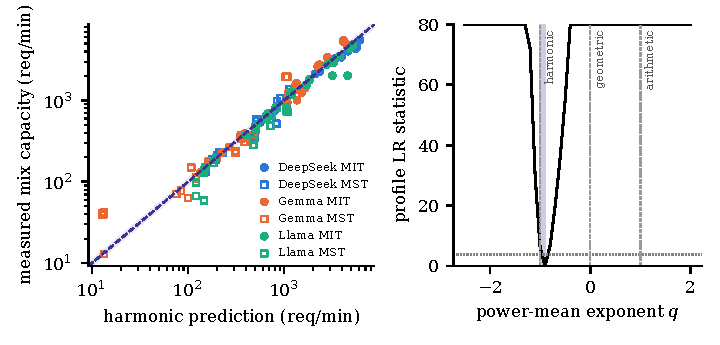
\includegraphics[width=\textwidth]{figures/fig_additivity}
  \caption{Left: measured mix capacity versus the harmonic prediction of Eq.~\eqref{eq:harmonic}
  (filled: MIT, hollow: MST; band: $\pm$10\,\%). Right: profile likelihood of the power-mean exponent
  $q$, with the Bayesian 95\,\% credible interval shaded.}
  \label{fig:additivity}
\end{figure}

\begin{figure}[t]
  \centering
  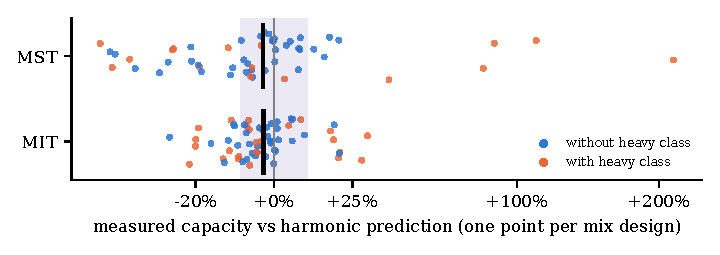
\includegraphics[width=\textwidth]{figures/fig_mit_mst}
  \caption{Departure of every mix design from the harmonic law in MIT and MST (black tick: mean;
  band: $\pm$10\,\%). Orange designs contain the heaviest request class.}
  \label{fig:mitmst}
\end{figure}

\subsection{Burst factor (RQ4)}
\label{sec:burst}

SCALE exposes a single currency based on the sustainable capacity and keeps the instantaneous capacity
$IK_{max}$ as a background safety threshold for bursts. We define the \emph{burst factor} of a request
class as the ratio of its instantaneous to its sustainable throughput,
\begin{equation}
  B_r \;=\; \frac{MIT_r}{MST_r},
  \label{eq:burst}
\end{equation}
i.e., how many times its sustainable rate a client may reach during a 2-minute burst. Since
$IK_r/SK_r = (IK_{max}/SK_{max})/B_r$, the sustainable and instantaneous Capacity Units rank and price
request classes identically if and only if $B_r$ is constant across classes. A constant burst factor is
therefore what justifies exposing one currency. RQ4 asks: \emph{is the burst factor constant across
request classes and deployments, and can it be used to size the burst allowance of a plan?}

\paragraph{The burst factor is nearly constant.} Across the \scaleBurstNCells request classes of the
three deployments, the median burst factor is \scaleBurstMedian (interquartile range
\scaleBurstQOne--\scaleBurstQThree; Table~\ref{tab:burst}, Fig.~\ref{fig:burst}), and the per-model
medians are almost identical: \scaleBurstDeepSeek for DeepSeek (95\,\% CrI
$[\scaleBurstDeepSeekLo, \scaleBurstDeepSeekHi]$), \scaleBurstGemma for Gemma
($[\scaleBurstGemmaLo, \scaleBurstGemmaHi]$) and \scaleBurstLlama for Llama
($[\scaleBurstLlamaLo, \scaleBurstLlamaHi]$). The model has no detectable effect
(ANOVA $p=\scaleBurstModelP$): the posterior ratio between the burst factors of any two models lies
within \scaleBurstPairCi of one (95\,\% CrI), and the probability that they are equivalent within
$\pm$10\,\% is at least \scaleBurstEquivMin. Moreover, \scaleBurstOnBand of the classes lie within
$\pm$15\,\% of their model's median. The burst factor is thus a highly portable property of a MoST-characterised deployment,
which strengthens the portability claim of RQ1 with a quantity that can be compared across models in
absolute terms, unlike $K$.

\paragraph{Systematic exceptions.} Once Gemma's two heaviest-output cells are set aside, the output
length has a clear effect ($p=\scaleBurstOutRobustP$): classes with short answers (1--100 output
tokens) tolerate larger bursts ($B=\scaleBurstShort$ vs.\ \scaleBurstRest, \scaleBurstShortRatio,
$p=\scaleBurstShortP$). The two Gemma cells with long inputs and long outputs reach $B$ up to
\scaleBurstMaxGemma; they coincide with the MST anomaly discussed in Sect.~\ref{sec:additivity}.
For mixes measured in both tests (\scaleBurstMixN designs), the measured burst factor exceeds the one
predicted from the class capacities by \scaleBurstMixErr on average, because mixes depart more from
additivity in MST than in MIT (Fig.~\ref{fig:burstmix}).

\paragraph{Implications for SCALE.} A single burst factor of about \scaleBurstMedian\ supports SCALE's
design choice of one user-facing currency: pricing bursts with sustainable Capacity Units mis-states
their instantaneous load by less than 15\,\% for \scaleBurstOnBand of the classes. It also gives a
direct rule for the Token Bucket: a plan with a sustainable rate $s$ can be granted a burst rate of up
to about $B\cdot s$ over 2-minute windows, with short-answer classes allowing about
\scaleBurstShortRatio more. Note that the illustrative capacity profile of the introduction
(30{,}000 requests per 30 minutes and 1{,}400 requests per minute, i.e., $B\approx\scaleBurstPaperExample$)
is far more conservative than the measured burst factor.

\begin{table}[t]
  \centering
  \caption{Burst factor $B=MIT/MST$ per model: median over the request classes (Bayesian 95\,\%
  credible interval), interquartile range, range, and share of classes within $\pm$15\,\% of the
  median.}
  \label{tab:burst}
  % Burst factor per model: median over the 20 request classes, spread and share within +-15 % of the median.
\begin{tabular}{lcccc}
\toprule
Model & Median $B$ [95\,\% CrI] & IQR & Range & Within $\pm$15\,\% \\
\midrule
DeepSeek-R1-Distill-Qwen-7B & 3.57 [3.49, 3.64] & 3.42--4.13 & 3.22--5.63 & 70\,\% \\
Gemma-7B & 3.56 [3.49, 3.65] & 3.40--3.90 & 2.99--11.64 & 75\,\% \\
Llama-3.1-8B-Instruct & 3.55 [3.48, 3.62] & 3.42--3.76 & 3.25--5.37 & 85\,\% \\
\midrule
All & 3.50 & 3.41--3.94 & -- & 77\,\% \\
\bottomrule
\end{tabular}

\end{table}

\begin{table}[t]
  \centering
  \caption{Burst factor per request class. Bold: more than 15\,\% away from the model's median.}
  \label{tab:burstmatrix}
  \resizebox{\textwidth}{!}{% Burst factor B = MIT/MST per request class (rows: input tokens, columns: output tokens).
\begin{tabular}{llrrrrr}
\toprule
 & & \multicolumn{5}{c}{Output tokens} \\
\cmidrule(lr){3-7}
Model & Input & 1-100 & 100-300 & 300-600 & 600-1000 & 1000-1500 \\
\midrule
\multirow{4}{*}{DeepSeek} & 600-1000 & \textbf{4.62} & 3.60 & 3.41 & 3.44 & 3.49 \\
 & 300-600 & 3.93 & \textbf{4.56} & 3.22 & 3.32 & 3.27 \\
 & 100-300 & \textbf{4.65} & \textbf{4.11} & \textbf{4.19} & 3.44 & 3.43 \\
 & 1-100 & \textbf{5.63} & 3.60 & 3.47 & 3.51 & 3.41 \\
\midrule
\multirow{4}{*}{Gemma} & 600-1000 & 3.45 & \textbf{4.08} & 3.48 & 3.62 & \textbf{11.64} \\
 & 300-600 & 3.64 & 3.65 & 3.43 & 3.28 & \textbf{6.02} \\
 & 100-300 & 3.98 & 3.87 & 3.41 & 3.26 & 3.40 \\
 & 1-100 & \textbf{4.24} & 3.37 & 3.46 & 3.37 & \textbf{2.99} \\
\midrule
\multirow{4}{*}{Llama} & 600-1000 & 3.91 & 3.56 & \textbf{4.13} & 3.52 & 3.29 \\
 & 300-600 & 3.58 & 3.71 & 3.43 & 3.41 & 3.25 \\
 & 100-300 & 3.99 & \textbf{5.37} & 3.48 & 3.39 & 3.43 \\
 & 1-100 & \textbf{4.69} & 3.55 & 3.45 & 3.50 & 3.41 \\
\bottomrule
\end{tabular}
}
\end{table}

\begin{figure}[t]
  \centering
  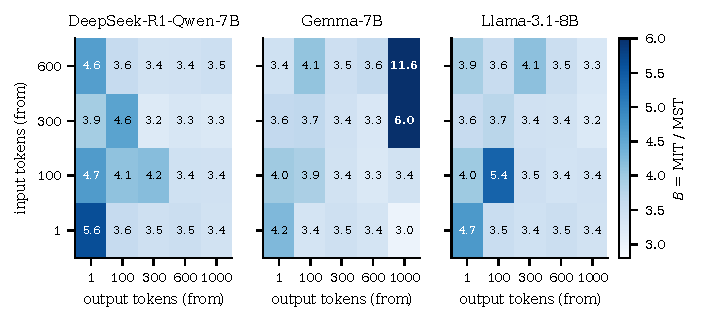
\includegraphics[width=\textwidth]{figures/fig_burst}
  \caption{Burst factor $B=MIT/MST$ of every request class (rows: input tokens; columns: output
  tokens; labels give the lower bound of each interval).}
  \label{fig:burst}
\end{figure}

\begin{figure}[t]
  \centering
  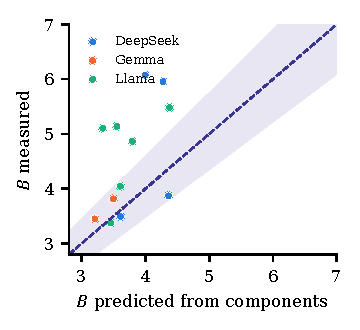
\includegraphics[width=0.5\textwidth]{figures/fig_burst_mix}
  \caption{Burst factor of mixes measured in both tests versus the value predicted from their classes
  (band: $\pm$15\,\%).}
  \label{fig:burstmix}
\end{figure}
